\documentclass[hyperref={pdfpagelabels=false}]{beamer}
\usepackage{animate}
\usepackage[spanish]{babel}
\usepackage{lmodern}


\title{Algoritmo de B\'usqueda Indexada}   
\author{Los Walo} 
\date{19 de julio del 2013} 


% Adicional intercala package{beamerthemeshadow} 
\usepackage{beamerthemeshadow}

\begin{document}
\begin{frame}
\titlepage %portada
\end{frame} 

\begin{frame}
\frametitle{\'Indice}
\tableofcontents
\end{frame} 


\section{Introducci\'on} 
\begin{frame}
\frametitle{Que es y en que consiste}
 \begin{itemize}
\item Algoritmo de B\'usqueda Recursivo.\\
\item Uso de Key o \'Indices.\\
\item Acci\'on de registrar ordenadamente la informaci\'on para elaborar su \'indice.\\
\item La indexaci\'on es un elemento fundamental para motores de b\'usqueda y las base de datos.\\
\item Es la manera mas eficiente de organizar y recuperar contenido de una base de datos.
\end{itemize}
\end{frame}


\section{Complejidad}
\begin{frame}
\frametitle{Complejidad} 
La complejidad es variable puede depender de:
\begin{itemize}
\item Algoritmo de Ordenamiento.
\item Uso de otros algoritmos de b\'usqueda. 
\item Forma de llenado de arreglos de indices.
\item Otros.
\end{itemize}
Calculo de la complejidad notaci\'on O(n):\\
\[
O(n)=7n^2+8n+n/c+1=n^2+log(n)=n^2
\]
\end{frame}

%Complejidad Peor caso O(n)
\begin{frame}
\frametitle{Complejidad (Peor caso O(n))}
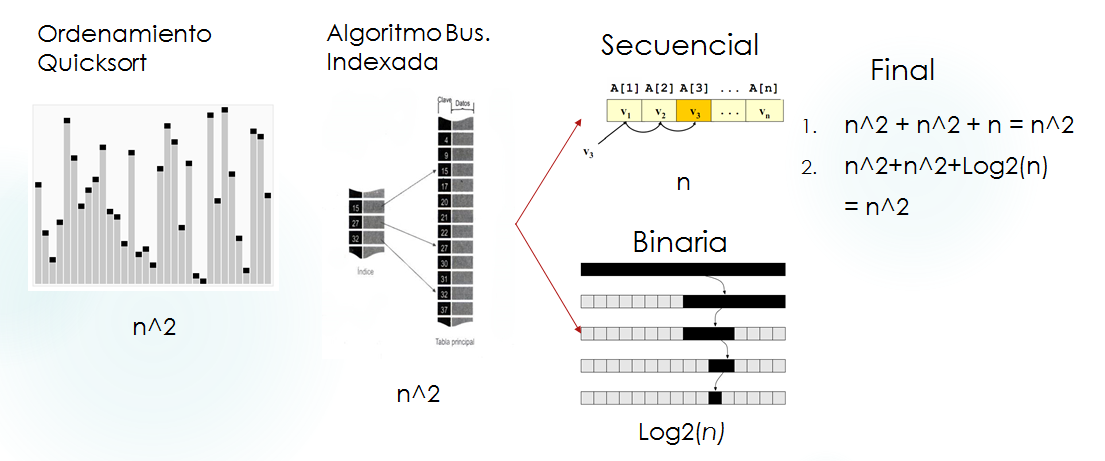
\includegraphics[width=1.1\textwidth]{casoPeor.png}
\end{frame}

%Complejidad caso medio O(n)
\begin{frame}
\frametitle{Complejidad (Caso Medio O(n))}
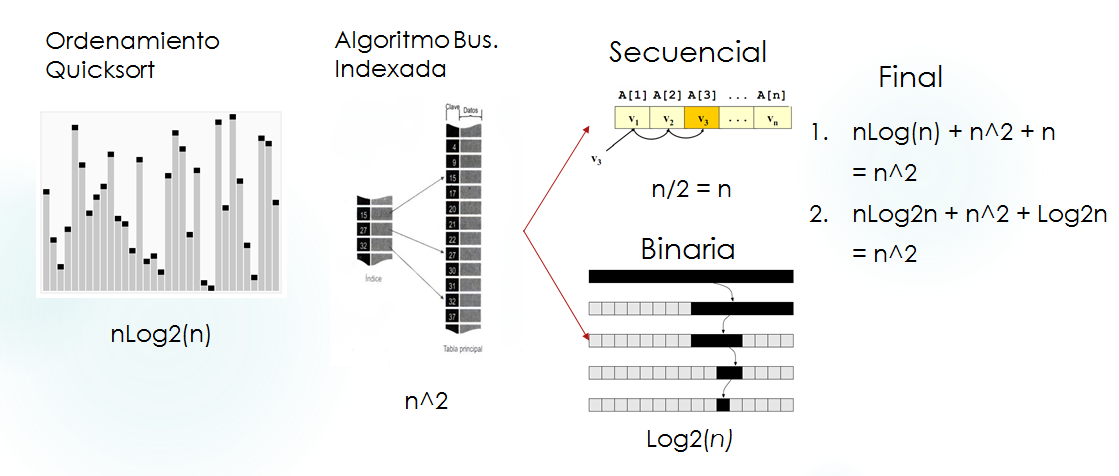
\includegraphics[width=1.1\textwidth]{casoMedio.png}
\end{frame}


\section{Como funciona}
\begin{frame}
\frametitle{Como funciona}
Mediante cada elemento del array \'indice se asocian grupos de elementos del array inicial.\\
Los elementos en el \'indice y en el array deben estar ordenados. 
El m\'etodo consta de dos pasos:\\

\begin{itemize}
\item Buscar en el array \'indice el intervalo correspondiente al elemento buscado.\\
\item Restringir la B\'usqueda a los elementos del intervalo localizado previamente.  
\end{itemize}

Se puede implementar la b\'usqueda binaria o secuencial en el array de \'indices y en el inicial.\\
Finaliza la b\'usqueda seg\'un las condiciones del algoritmo de b\'usqueda sub-utilizado (Binario/Secuencial).
\end{frame}

\begin{frame}
\frametitle{Ejemplos (B\'usqueda Secuencial)}
\includegraphics[width=1.0\textwidth]{busqSecuencial.png}
\end{frame}

\begin{frame}
\frametitle{Ejemplos (B\'usqueda Binaria)}
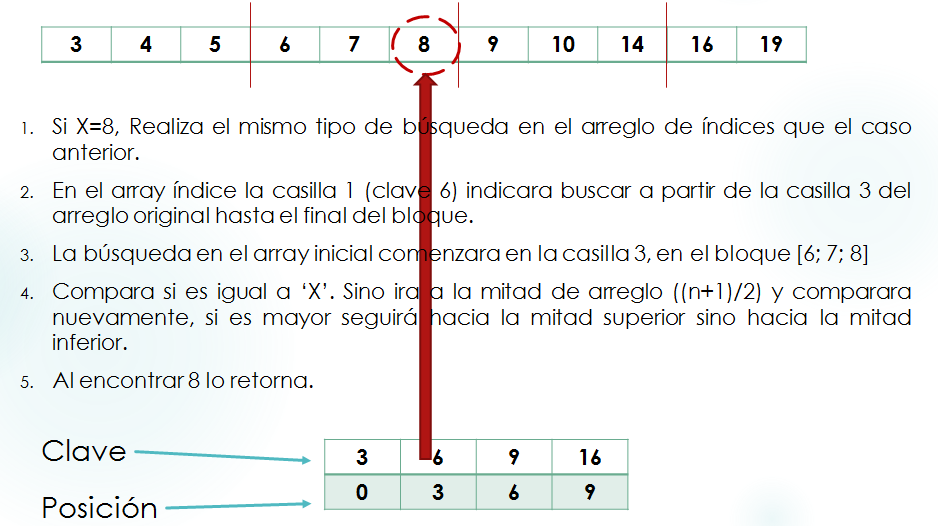
\includegraphics[width=1.0\textwidth]{busqBin.png}
\end{frame}

\begin{frame}
\frametitle{Tabla de medici\'on}
\begin{tabular}{|c|c|c|c|}
\hline
\textbf{A[]} & \textbf{1.000} & \textbf{10.000} & \textbf{100.000} \\
\hline Tiempo(s)& 0.296 seg.&0,643 seg.& 6.079 seg.\\ \hline
\end{tabular}
\end{frame}

\section{Cuando Ocupamos B\'usqueda Indexada}
\begin{frame}
\frametitle{Cuando ocupamos B\'usqueda Indexada}
\begin{itemize}
\item Conveniente para archivos con mediana volatilidad, actividad variable y tama\~no estable.
\item Para N muy grandes (porque?)
\item En lugares donde se presente el ingreso de datos (registros) sin ning\'un tipo de orden especifico
\item Ejemplos: Spip (que es Spip?)
\end{itemize}
\end{frame}

\begin{frame}
\frametitle{Ejemplo de Indexaci\'on para textos}
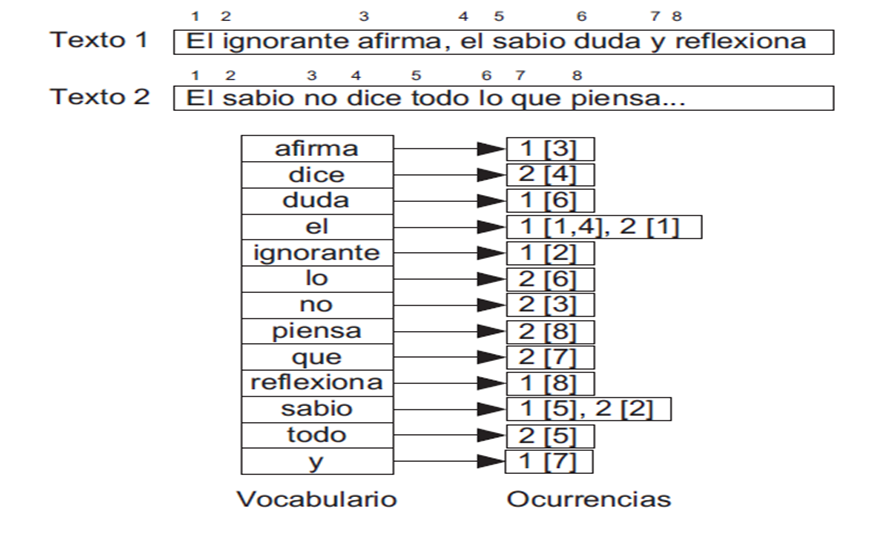
\includegraphics[width=1.0\textwidth]{busqText.png}
\end{frame}

\section{Ventajas y desventajas}
\begin{frame}

Ventajas

\begin{itemize}
\item Procesar archivo secuencialmente por orden l\'ogico o al azar.
\item Se hace una b\'usqueda en una tabla de \'indices peque\~na y luego en una parte reducida de la tabla original de registros.
\end{itemize}

Desventajas

\begin{itemize}
\item Implica un aumento en la cantidad de espacio requerido.
\item El uso de una lista de \'indices da una gran sobrecarga de espacio y tiempo para los apuntadores usados en b\'usquedas de registros.
\item La inserci\'on en una tabla secuencial indexada es dif\'icil.
\item Los registros deben ser de longitud fija.
\end{itemize}
\end{frame}

\section{Conclusiones}
\begin{frame}
\frametitle{Conclusiones}
\begin{itemize}
\item Es el m\'etodo de B\'usqueda mas r\'apido, sin embargo necesita ocupar otro tipo de b\'usqueda.
\item Sera m\'as r\'apida cuando los n sean muy grandes.
\item Es uno de los m\'etodos de b\'usqueda m\'as usado por los motores de b\'usqueda de Internet.
\item Su eficacia se observa en la b\'usqueda en archivos de gran magnitud.
\end{itemize}
\end{frame}

\end{document}